\documentclass[t]{beamer}
\usecolortheme[RGB={0,114,197}]{structure} 
\usetheme{Ilmenau} 
\usepackage{tikz}
\usepackage{multicol}

\title{Software-Ontwerp}
\subtitle{Iteratie 4}
\author{Castel D. - Devlieghere J. - Pante S.}
\institute{KU Leuven}

\begin{document}

\frame{\titlepage} 
\begin{frame}{Inhoud}
\begin{multicols}{2}
\tableofcontents
\end{multicols}
\end{frame}



\section{Inleiding} 

\subsection{Rolverdeling}
\begin{frame}{Rolverdeling}
\begin{multicols}{2}
\tableofcontents[currentsection]
\end{multicols}
\end{frame}

\begin{frame}{Rolverdeling}
Afgelopen iteratie:
\begin{itemize}
	\item Lead Designer: Vincent Reniers
	\item Lead Tester: Jonas Devlieghere
	\item Domain Modeler: Dieter Castel
\end{itemize}
Komende iteratie:
\begin{itemize}
	\item Lead Designer: Stefan Pante
	\item Lead Tester: Dieter Castel
	\item Domain Modeler: Jonas Devlieghere
\end{itemize}
\end{frame}

\subsection{Werkverdeling}

\begin{frame}{Werkverdeling}
\begin{figure}[h!]
	\center
	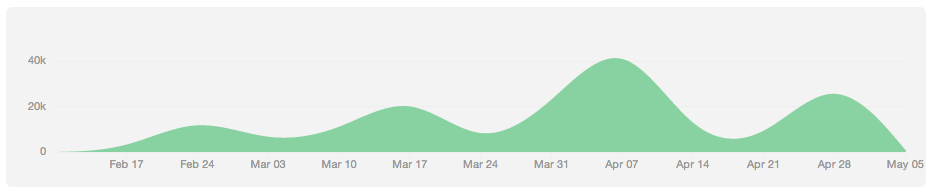
\includegraphics[width= 0.9\linewidth]{img/github.png}
	\caption{Commit history doorheen de iteraties}
\end{figure}

\end{frame}

\section{Tests}

\begin{frame}{Testen}
\begin{multicols}{2}
\tableofcontents[currentsection]
\end{multicols}
\end{frame}

\begin{frame}{Test Coverage}
\begin{figure}[h!]
	\center
	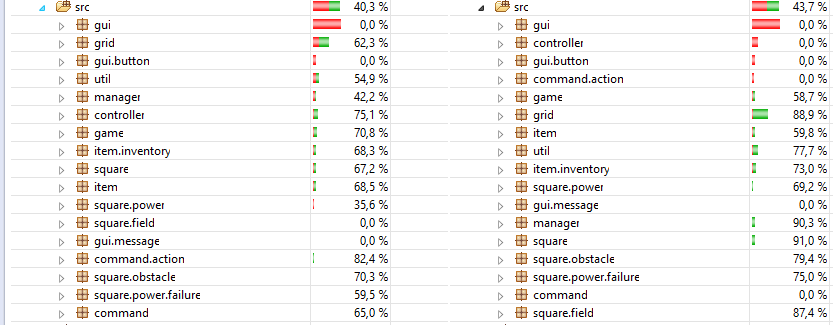
\includegraphics[width= 0.9\linewidth]{img/coverage.png}
	\caption{EclEmma test coverage}
\end{figure}
\end{frame}

\section{Nieuwigheden deze iteratie}

\subsection{Grid Builder}
\begin{frame}{Grid Builder}
\begin{figure}
	\center
	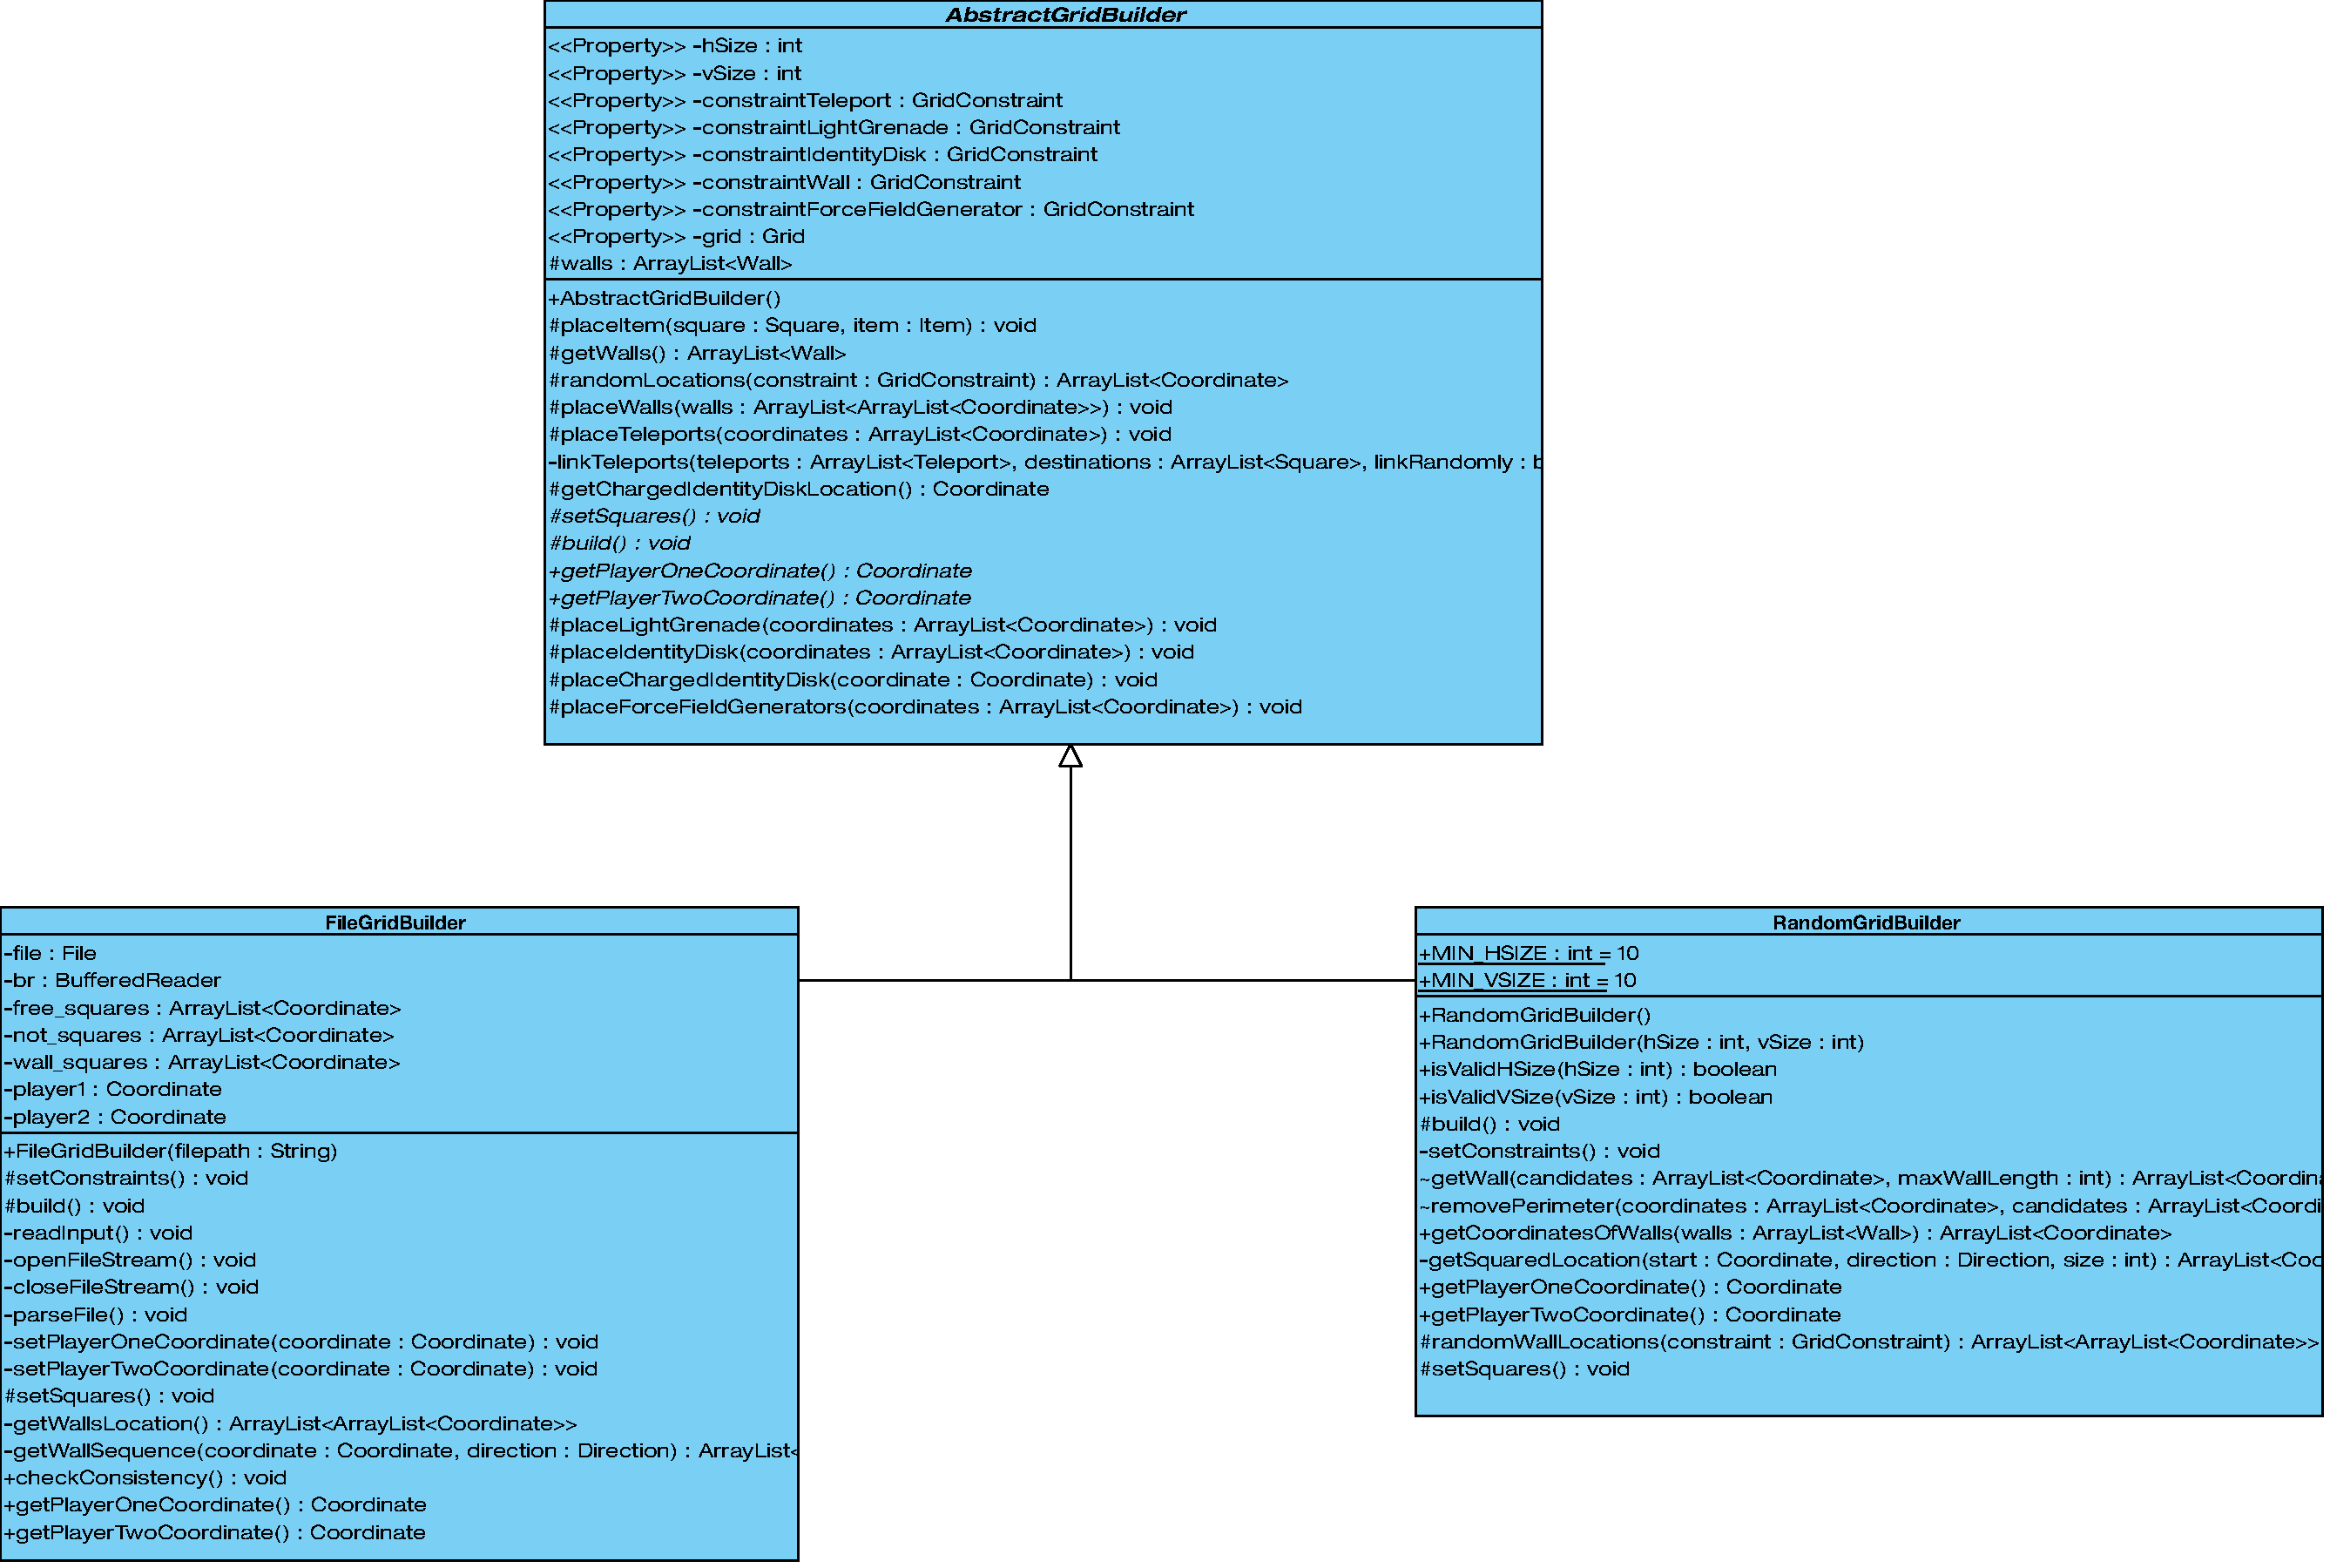
\includegraphics[width= 0.7\linewidth]{img/gridbuilder.pdf}
\end{figure}
\end{frame}

\subsection{Power Failures}
\begin{frame}{Power Failures}
\begin{figure}
	\center
	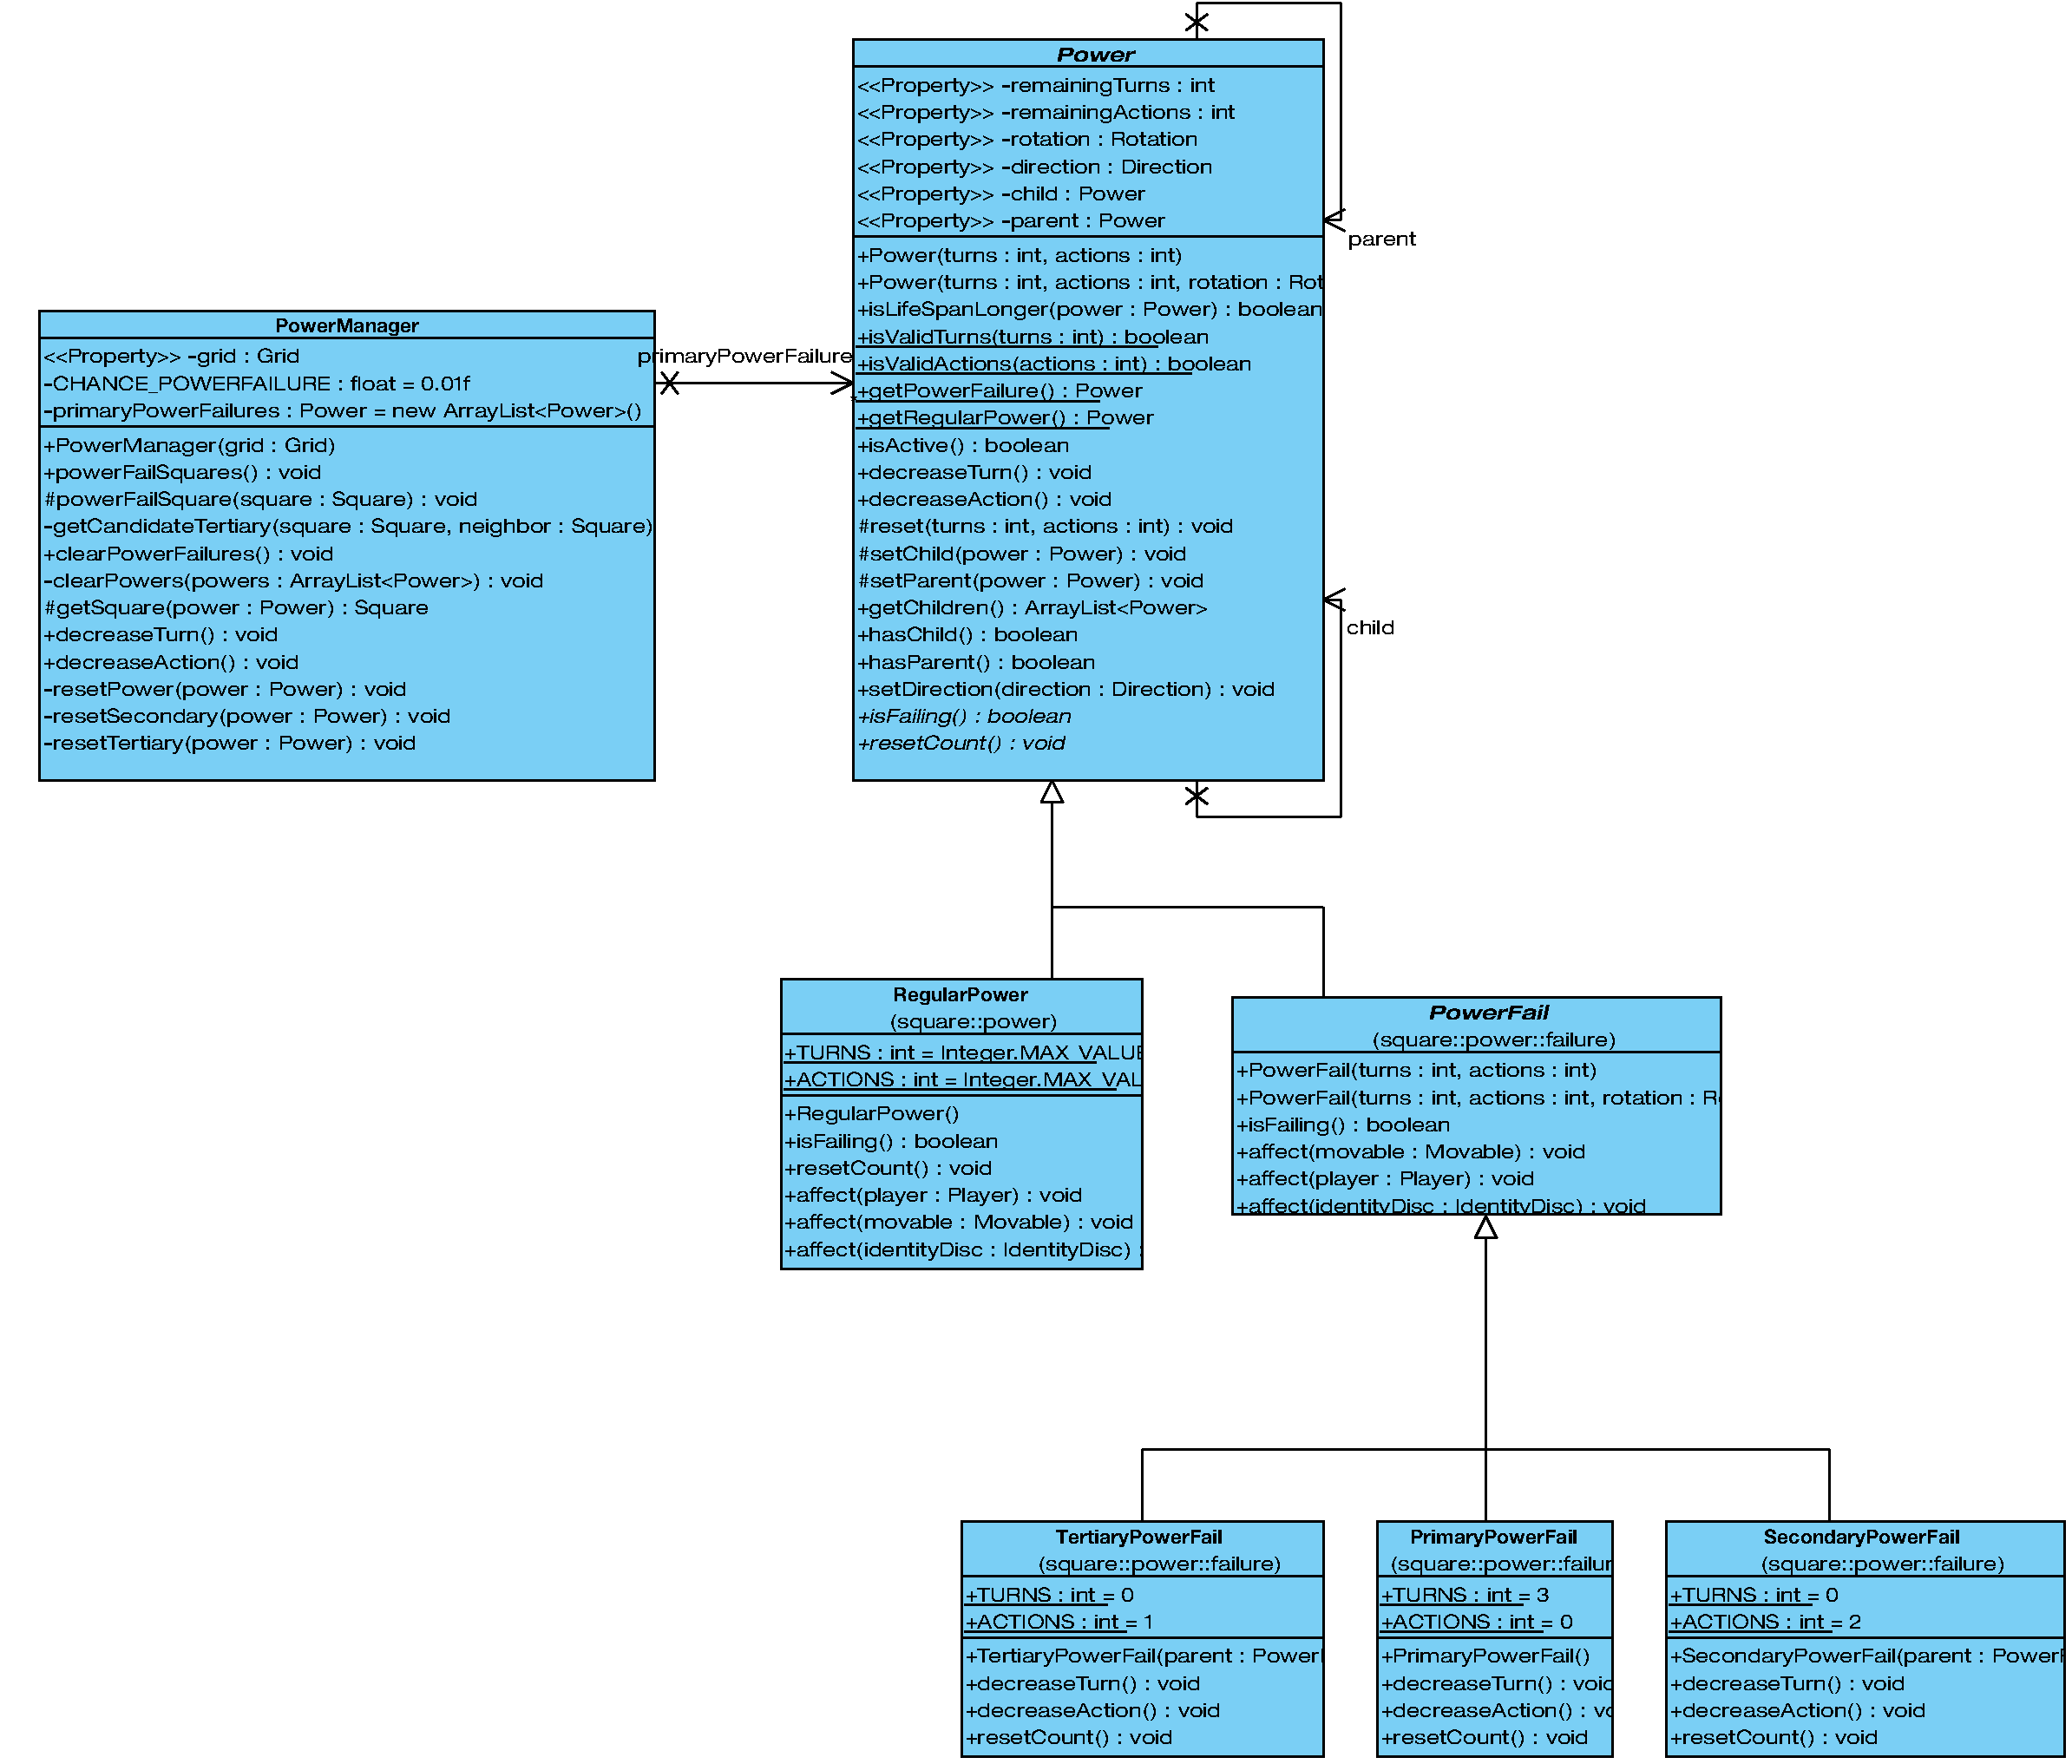
\includegraphics[width= 0.65\linewidth]{img/powerfail.pdf}
\end{figure}
\end{frame}


\subsection{Force Fields}
\begin{frame}{Force Fields}
\begin{figure}
	\center
	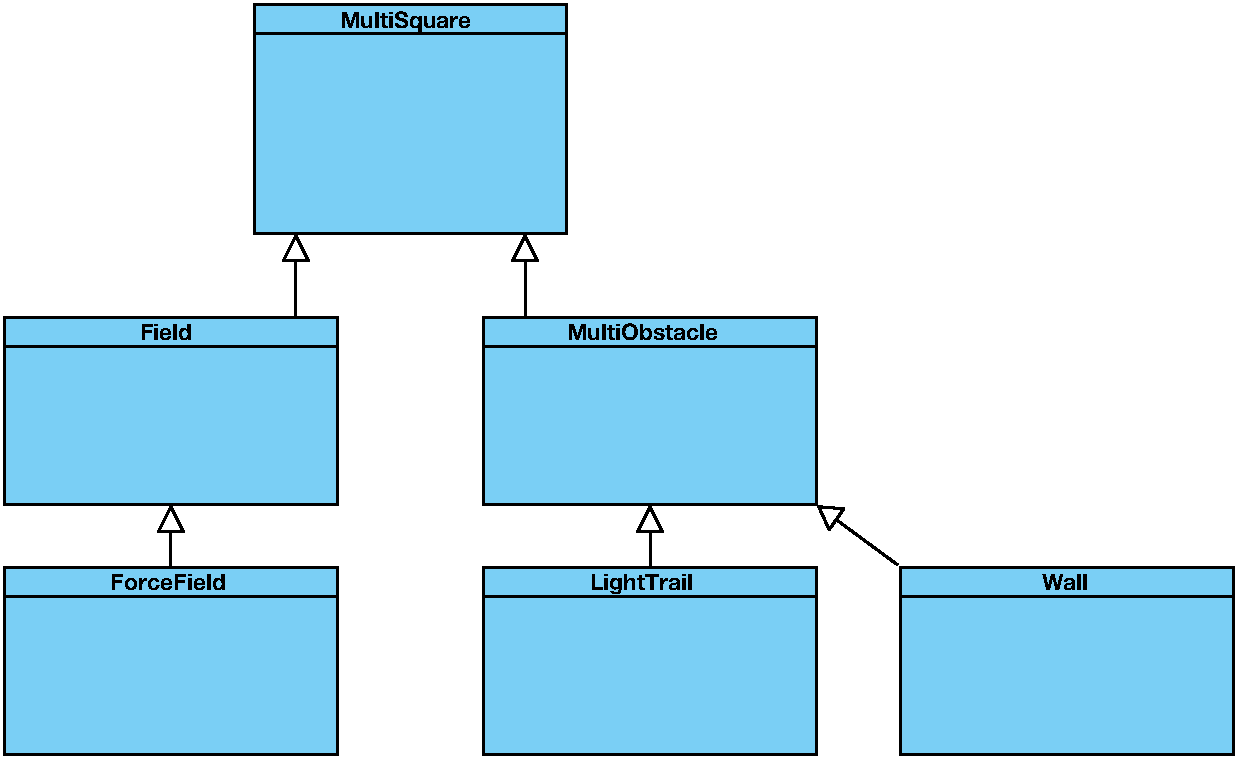
\includegraphics[width= 0.6\linewidth]{img/forcefield.pdf}
	\caption{Fields en Force Fields}
\end{figure}
\end{frame}


\subsubsection{Force Field Generators}
\begin{frame}{Force Field Generators}
\begin{figure}
	\center
	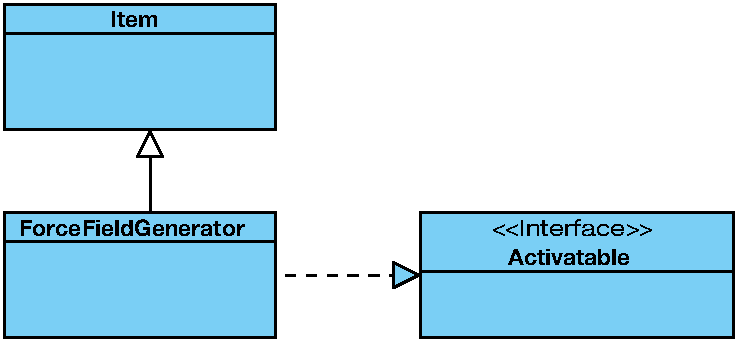
\includegraphics[width= 0.5\linewidth]{img/forcefieldgenerator.pdf}
	\caption{Force Field Generators}
\end{figure}
\begin{itemize}
	\item Force Field Generators zijn \textit{items}
	\item Force Field Generators zijn \textit{activatable}
\end{itemize}
\end{frame}

\subsubsection{Force Field Manager}
\begin{frame}{Force Field Manager}
\begin{multicols}{2}
\begin{figure}
	\center
	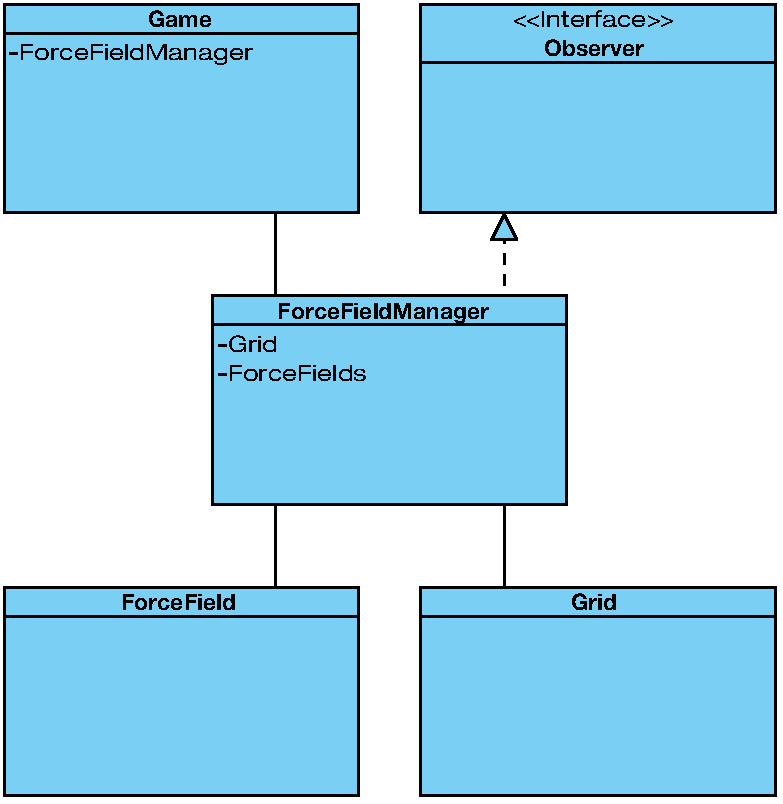
\includegraphics[width= 0.9\linewidth]{img/forcefieldmanager.pdf}
	\caption{Force Field Generators}
\end{figure}

\begin{itemize}
	\item Herkent aan de hand van het Grid welke Force Fields geactiveerd kunnen worden
	\item Gekoppeld met elk force field
	\item Generatoren zijn niet gekoppeld met velden zelf
	\item Observeert acties en schakelt velden aan en uit
\end{itemize}
\end{multicols}
\end{frame}


\subsection{MovableEffect}
\begin{frame}{Effecten}
\begin{multicols}{2}
\begin{minipage}{\columnwidth}
\begin{figure}
	\center
	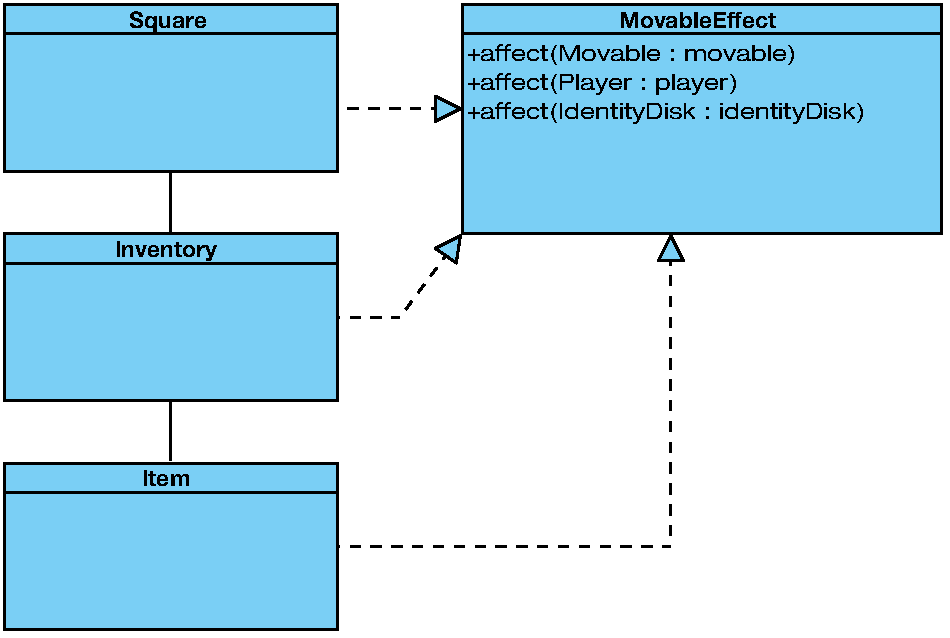
\includegraphics[width=\linewidth]{img/composite.pdf}
	\caption{Ge\"{i}nspireerd door Composite Pattern}
\end{figure}
\end{minipage}
\begin{minipage}{\columnwidth}
\begin{itemize}
	\item Zelfde interface voor complex object (\textit{square/inventory}) als voor primitief object (\textit{item}) 
	\item Gecombineerd met \textit{double dispatch} voor onderscheid van effect op \textit{item} en op \textit{player}
\end{itemize}
\end{minipage}


\end{multicols}
\end{frame}

\section{Aanpassingen}

\subsection{Activatable}


\subsection{Movable}
\begin{frame}
\begin{multicols}{2}
\begin{minipage}{\columnwidth}
\begin{figure}
	\center
	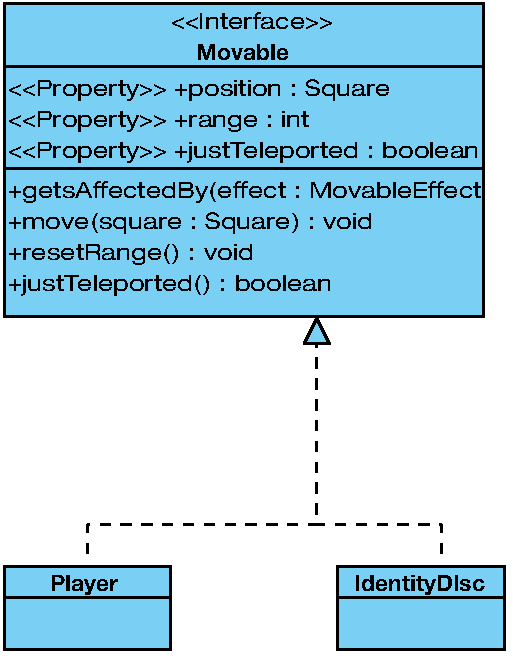
\includegraphics[width=\linewidth]{img/movable}
\end{figure}
\end{minipage}
\begin{minipage}{\columnwidth}
\begin{itemize}
	\item Interface movable zorgt ervoor dat alle actoren met zelfde methode kunnen bewegen 
	\item Ge\"implementeerd door Player en IdentityDisc, het verschillende gedrag bij powerfailures, teleports wordt afgehandeld door effecten.
\end{itemize}
\end{minipage}
\end{multicols}
\end{frame}
\subsection{Commands}
\begin{frame}{Command Pattern}
\begin{figure}
	\center
	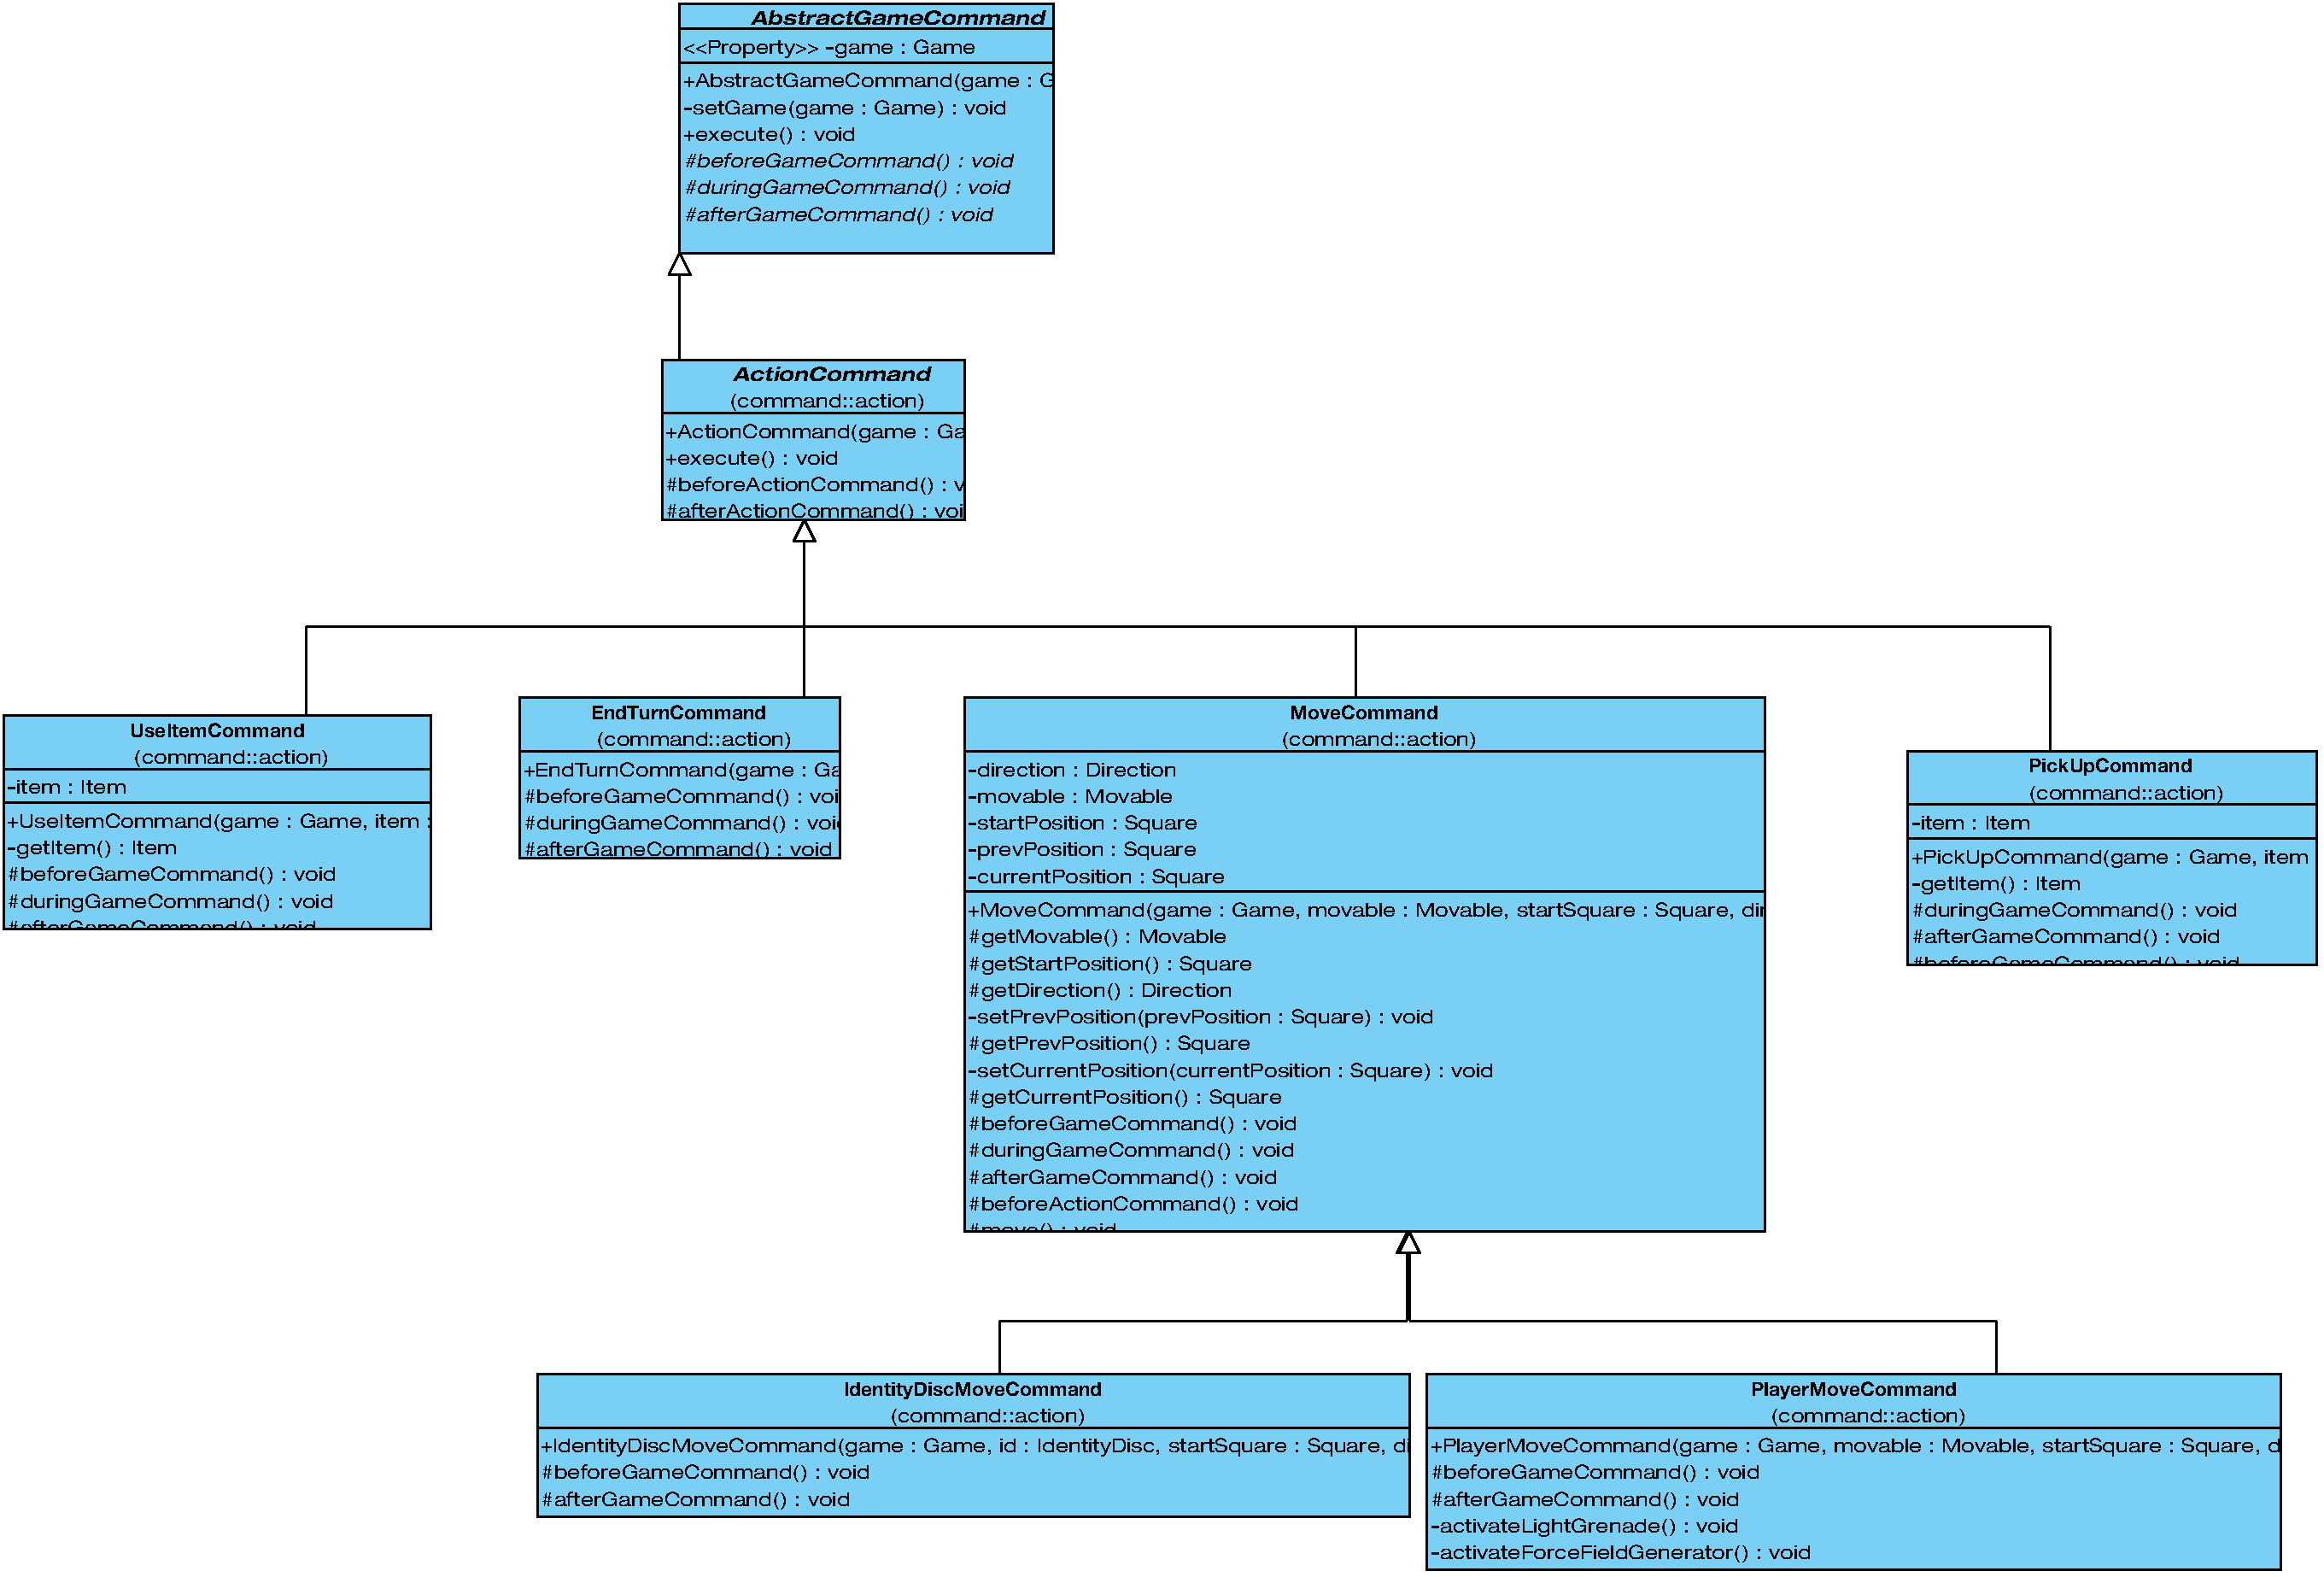
\includegraphics[width= 0.8\linewidth]{img/Command_pattern.pdf}
\end{figure}	
\end{frame}


\begin{frame}{Move Handler}
\begin{multicols}{2}
\begin{minipage}{\columnwidth}
\begin{figure}
	\center
	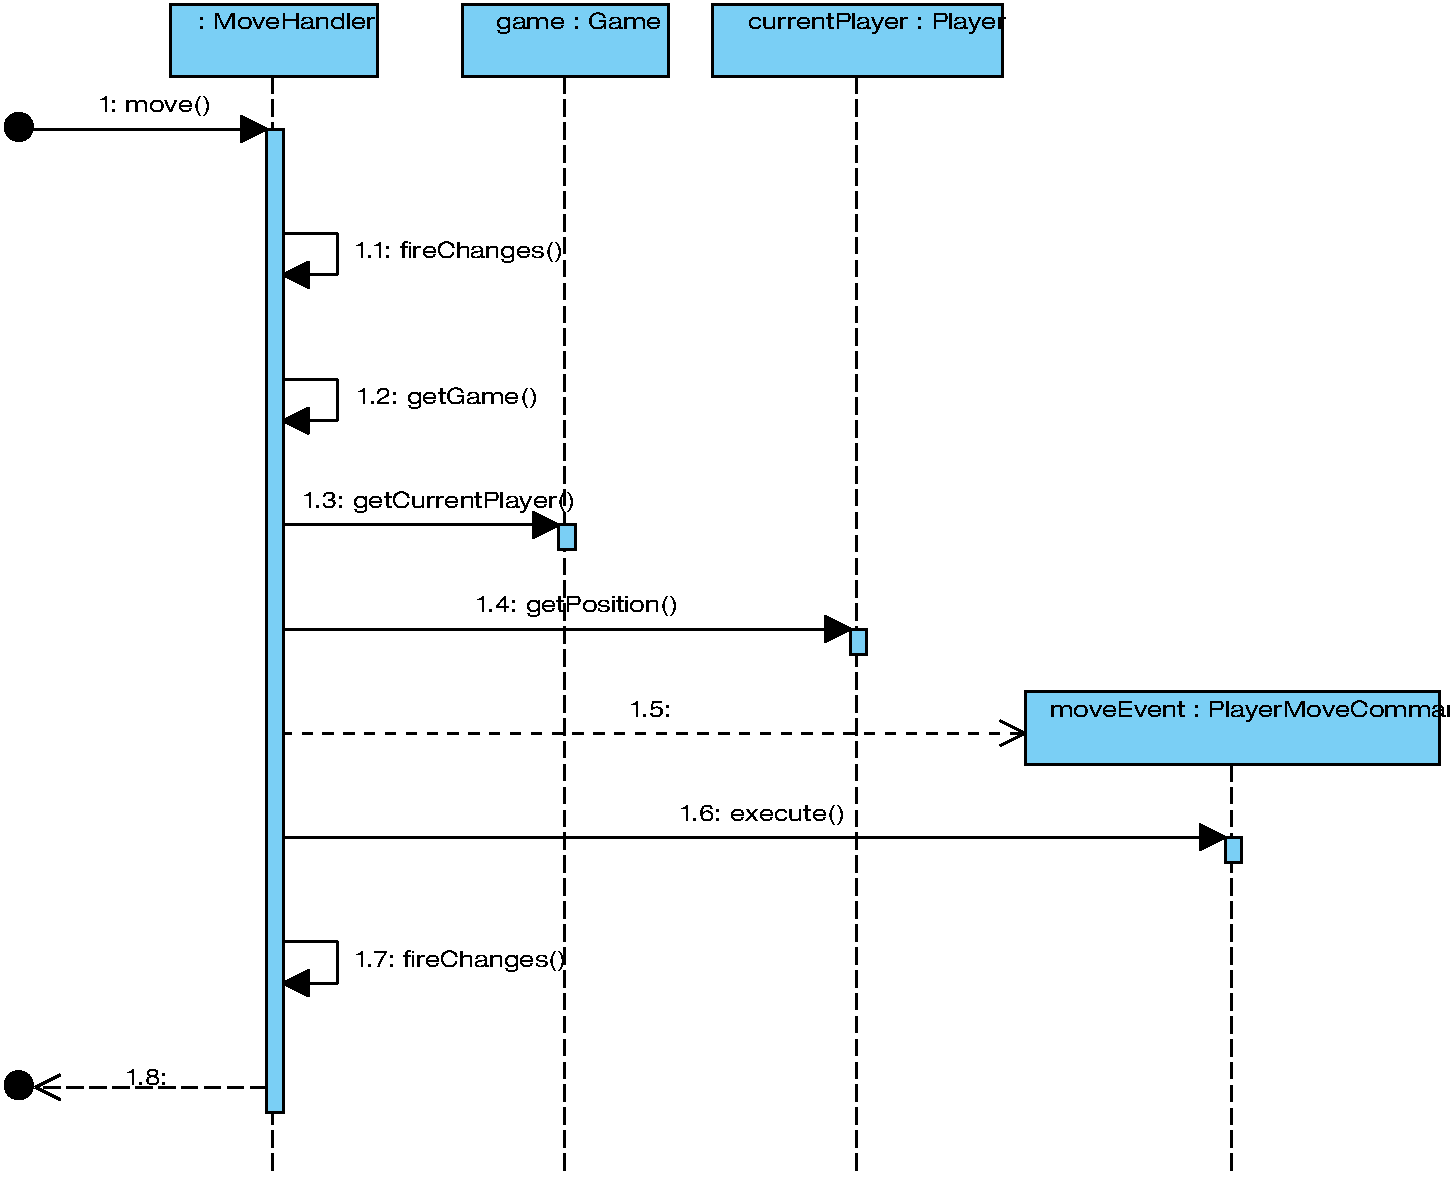
\includegraphics[width=\linewidth]{img/movehandler}
\end{figure}
\end{minipage}
\begin{minipage}{\columnwidth}
\begin{itemize}
	\item de Handlers gebruiken Commands voor de eigenlijke uitvoering van de actie.
	\item Zorgt voor sterke encapsulatie binnen de Handlers.
\end{itemize}
\end{minipage}
\end{multicols}
\end{frame}

\begin{frame}{Move Command}
\begin{figure}
	\center
	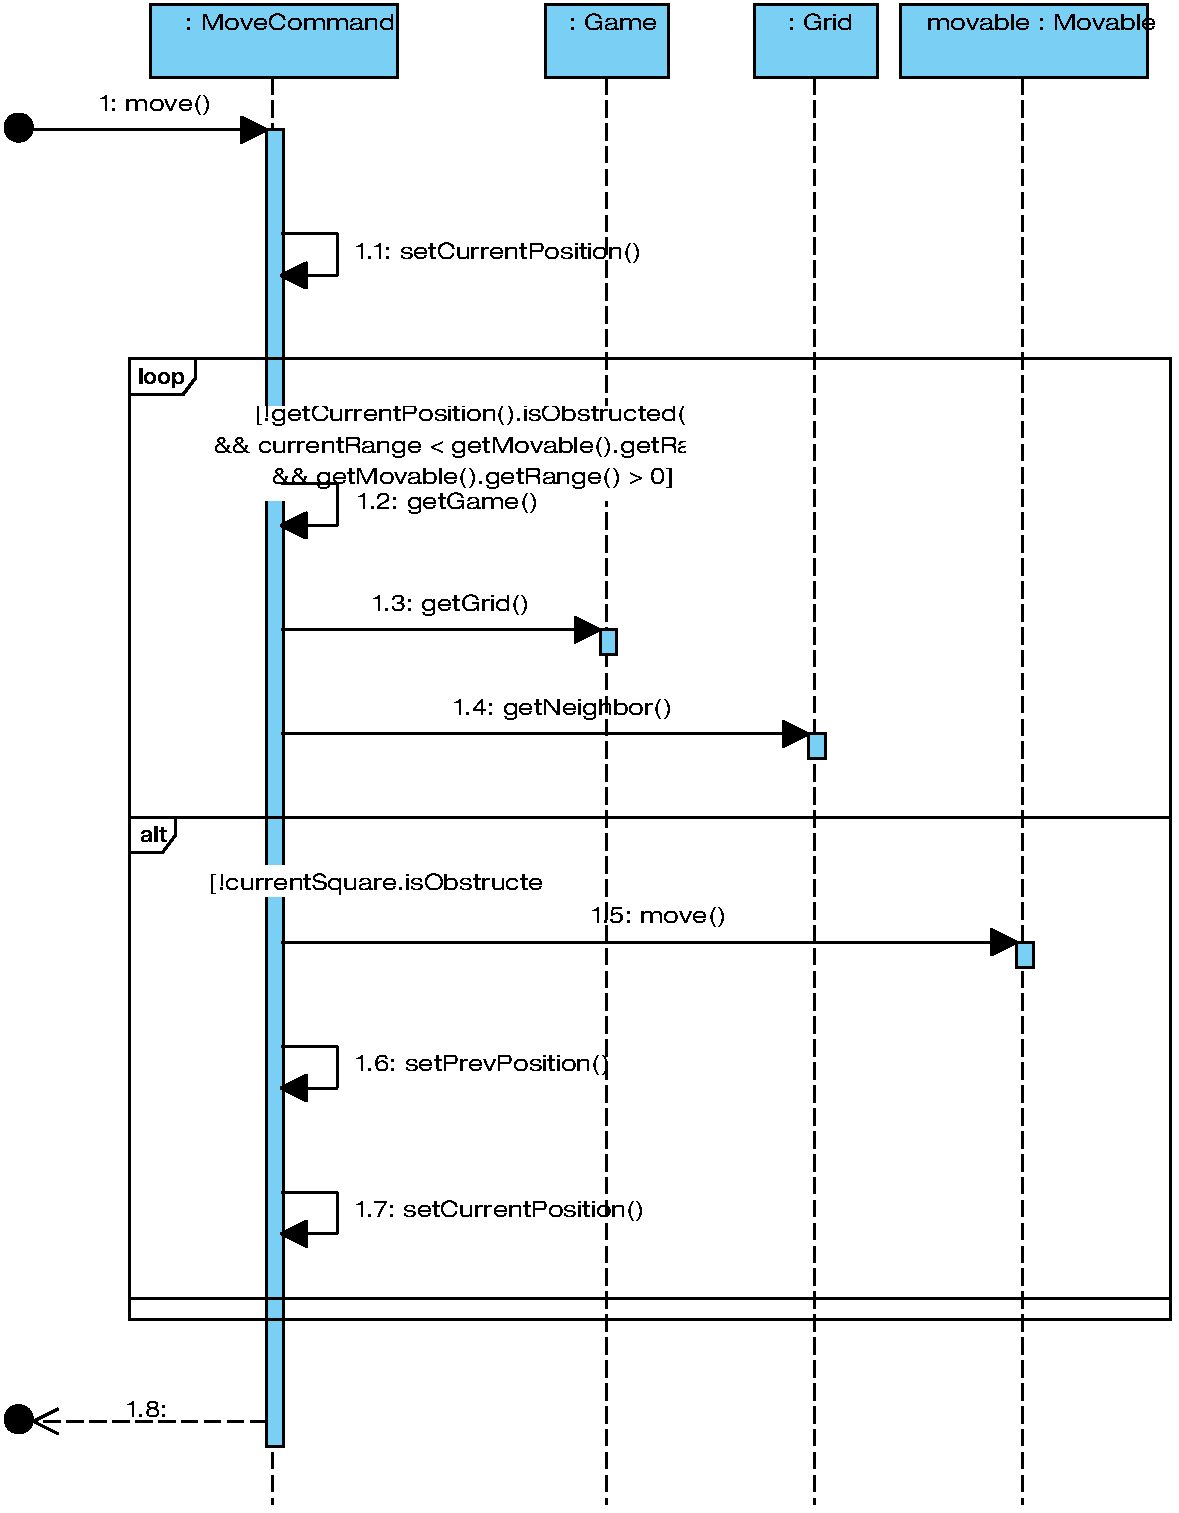
\includegraphics[scale=0.22]{img/movecommand}
\end{figure}
\end{frame}


\section{Slot}
\begin{frame}{Besluit}

\begin{center}
\begin{figure}
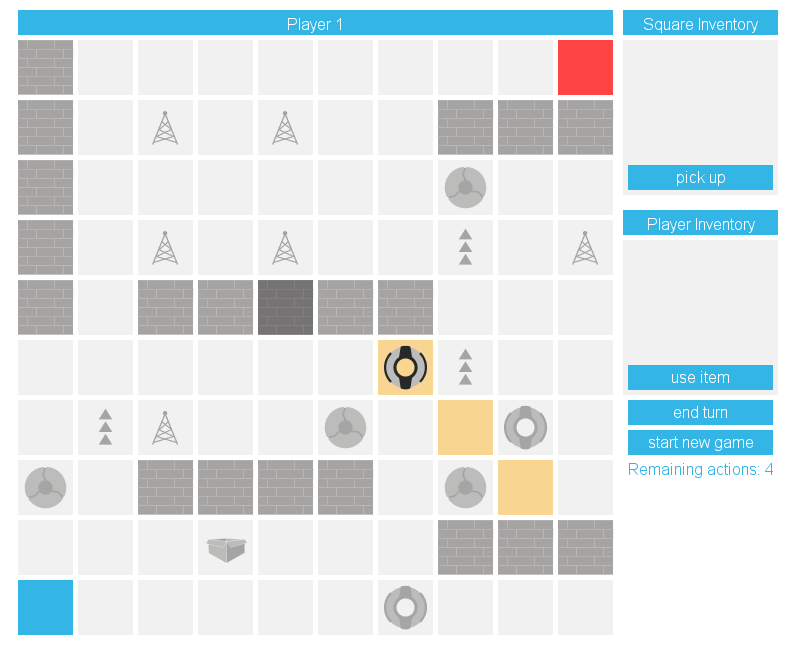
\includegraphics[scale=0.2]{img/game}
\end{figure}
\vspace{0.1in}
Bedankt voor uw aandacht.
\end{center}
\end{frame}

\end{document}
